\chapter{Einleitung}

    Dieser Projektbericht ist im Rahmen der Cross Innovation Class 2022 entstanden.

\section{Cross Innovation Class}

    Die Cross Innovation Class, kurz CIC, ist eine von der Hamburg Kreativ Gesellschaft organisierte Veranstaltung in Kooperation mit Universitäten und Fachhochschulen des Hamburger Umlands.
    Idee der CIC ist es Studierende verschiedener Fachrichtungen unterschiedlicher Universitäten ein Semester lang in interdisziplinären Teams an Projekten zusammenarbeiten.

    Teilnehmen konnten Studierende des Studiengangs Stadtplanung der Hafencity Universität Hamburg, der Studiengänge Produkt- und Interior-Designer der Akademie Mode \& Design des Standorts Hamburg und der Studiengänge Informatik, Technische Informatik, Wirtschaftsinformatik, Smart Technology und IT-Ingenieurwesen der Fachhochschule Wedel.

    Die Cross Innovation Class lief dabei dieses Jahr unter dem Thema Resilient Cities. In Bezug auf dieses Oberthema wurden fünf Partnerunternehmen ausgesucht, die jeweils eine Fragestellung mit in die CIC gebracht haben.


    \vspace{1em}
    \framebox[\textwidth]{
        \begin{minipage}{\textwidth-1em}
            \vspace{.4em}
            \textbf{Resilient Cities}
            \\ \\
            Resilienz, ein wichtiger Faktor in vielen Lebensbereichen.
            Ein Attribut das Anpassungsfähigkeit und einen standhaften Umgang mit Krisen beschreibt.
            Neben persönlicher und ökonomischer Resilienz übernimmt Resilienz auch eine immer wichtiger werdende Rolle im Blick auf Gemeinden und Städte.
            Vorallem im Bezug auf Extremwetterereignisse und dem immer weiter voranschreitenden Klimawandel braucht es neue Ideen und Konzepte.
            \\ \\
            Daher gibt es viele Bestrebungen auf globaler, europäischer und nationaler Ebene dieses Thema voranzubringen. Eine Institution ist der Urban Resilience Club, der Urbane Resilienz wie folgt definiert:
            \\
            \enquote{Urban Resilience - The measurable ability of any urban system, with its inhabitants, to maintain continuity through all shocks and stresses, while positively adapting and transforming toward sustainability.}\footnote{\url{https://urbanresiliencehub.org/what-is-urban-resilience/}}
            \\
        \end{minipage}
    }
    \vspace{1em}
    
    Partner dieses Jahr waren die Stadt Frankfurt mit der Stabsstelle Digitalisierung, die ACO Gruppe, Hamburg Marketing, Hamburg Institute for Innovation, Climate Protection and Circular Economy (HiiCCE) und das Wald Stadt Labor Iserlohn. \\

    Fünf Teams, jeweils bestehend aus Studierenden jeder Universität und einem Praxispartner durchliefen über knapp 12 Wochen ein Design Thinking Prozess, der 

    \begin{figure}[h]
        \begin{center}
            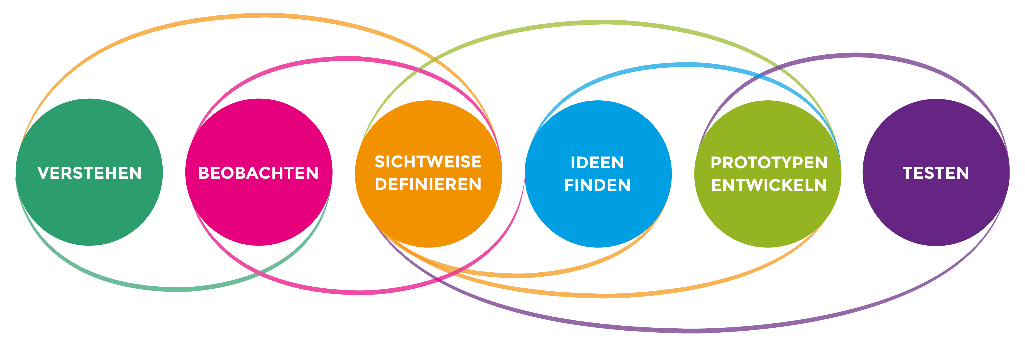
\includegraphics[width=12cm]{media/00_introduction/design_thinking_2.png}
        \end{center}
        \caption{Der Design-Thinking-Prozess\protect\footnote{Quelle: Design Thinking Workshop CrossInnovationClass}}
        \label{fig:dt_2}
    \end{figure}

    \begin{figure}[h]
        \begin{center}
            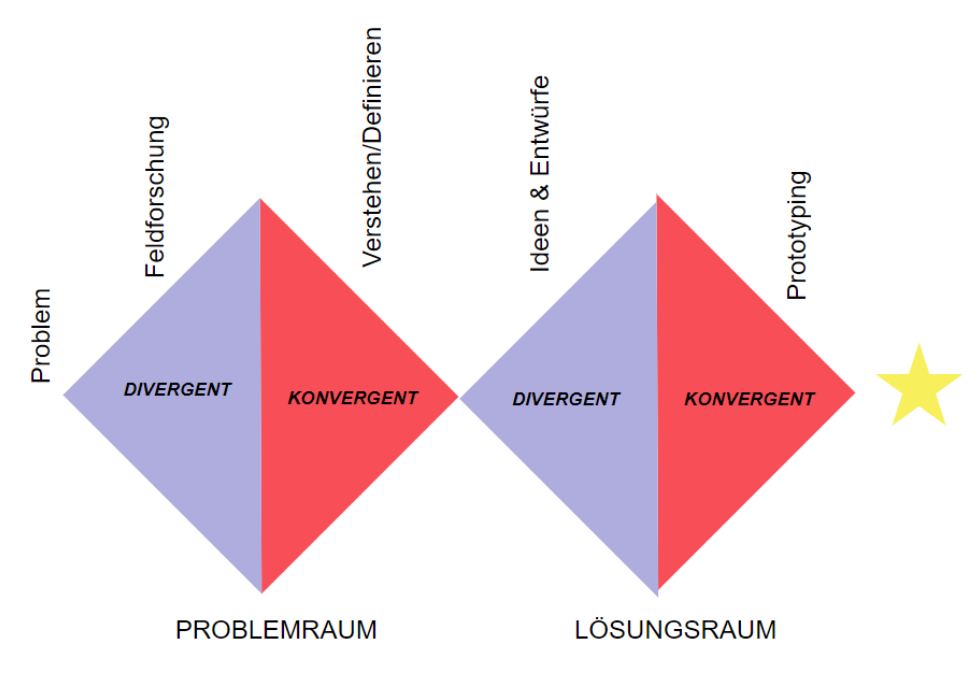
\includegraphics[width=12cm]{media/00_introduction/design_thinking_1.png}
        \end{center}
        \caption{Denkmodell \enquote{Double Diamond}\protect\footnotemark[\value{footnote}]}
        \label{fig:dt_1}
    \end{figure}
    

    \vspace{1em}
    \framebox[\textwidth]{
        \begin{minipage}{\textwidth-1em}
            \vspace{.4em}
            \textbf{Design Thinking}
            \\ \\
            Design Thinking ist ein Prozess zur Ideenfindung und -entwicklung.
            Dabei steht der Mensch im Mittelpunkt der mit einem Problem konfrontiert ist.
            
            Abbildung\,\ref{fig:dt_2} Zeigt die sechs Phasen, sowie die 

            In vielen Veranstaltungen der CIC ist uns der \enquote{Double Diamond} (Abbildung\,\ref{fig:dt_1}) begegnet, denn auch der Ablauf der Cross wurde in einem solchen Rahmen strukturiert.
            \vspace{.4em}
        \end{minipage}
    }
    \vspace{1em}

    Dieses Format stellt im Vergleich zu den sonst eher theoretischeren oder fachspezifischeren Veranstaltungen eine willkommene Ergänzung da.

    \subsection{Ablauf der CIC}

        Das Projekt wurde in drei große Phasen eingeteilt, Konzept, Entwurf und Prototyping.

        Neben einem KickOff zu Beginn gab es am Ende jeder Phase eine Feedback Runde mit der gesamten Class.
        
        In der KickOff Veranstaltung haben sich die Praxispartner und ihre Fragestellung vorgestellt und wir haben unser Team kennengelernt.



        Zusätzlich wurde allen Interessierten vor der Abschlussveranstaltung ein sehr lehrreiches Pitch-Training angeboten.

        Wie sind die Teams enstanden, was hatten wir für (Regel)Termine, wie viel Zeit hatten wir für die unterschiedlichen Aufgaben, etc.
        Skizzierung des CiC-Prozesse.

    \subsubsection{Projektphasen}

        \begin{center}
            \begin{tabular}{ |c|c|c| } 
                \hline
                \printdate{2022-04-08} & Kick-Off \\
                \hline
                \hline
                \printdate{2022-04-11} - \printdate{2022-04-21} & Analyse \& Konzept Phase \\ 
                \hline
                \printdate{2022-04-25} - \printdate{2022-05-06} & Entwurfsphase \\
                \hline
                \printdate{2022-05-09} - \printdate{2022-06-23} & Prototyping \& Modellbau Phase \\
                \hline                
                \hline
                \printdate{2022-06-30} & Abschlussveranstaltung \\
                \hline
            \end{tabular}
        \end{center}


\section{Team Frankfurt}

        
        Unser Team 

        \begin{figure}[h]
            \begin{center}
                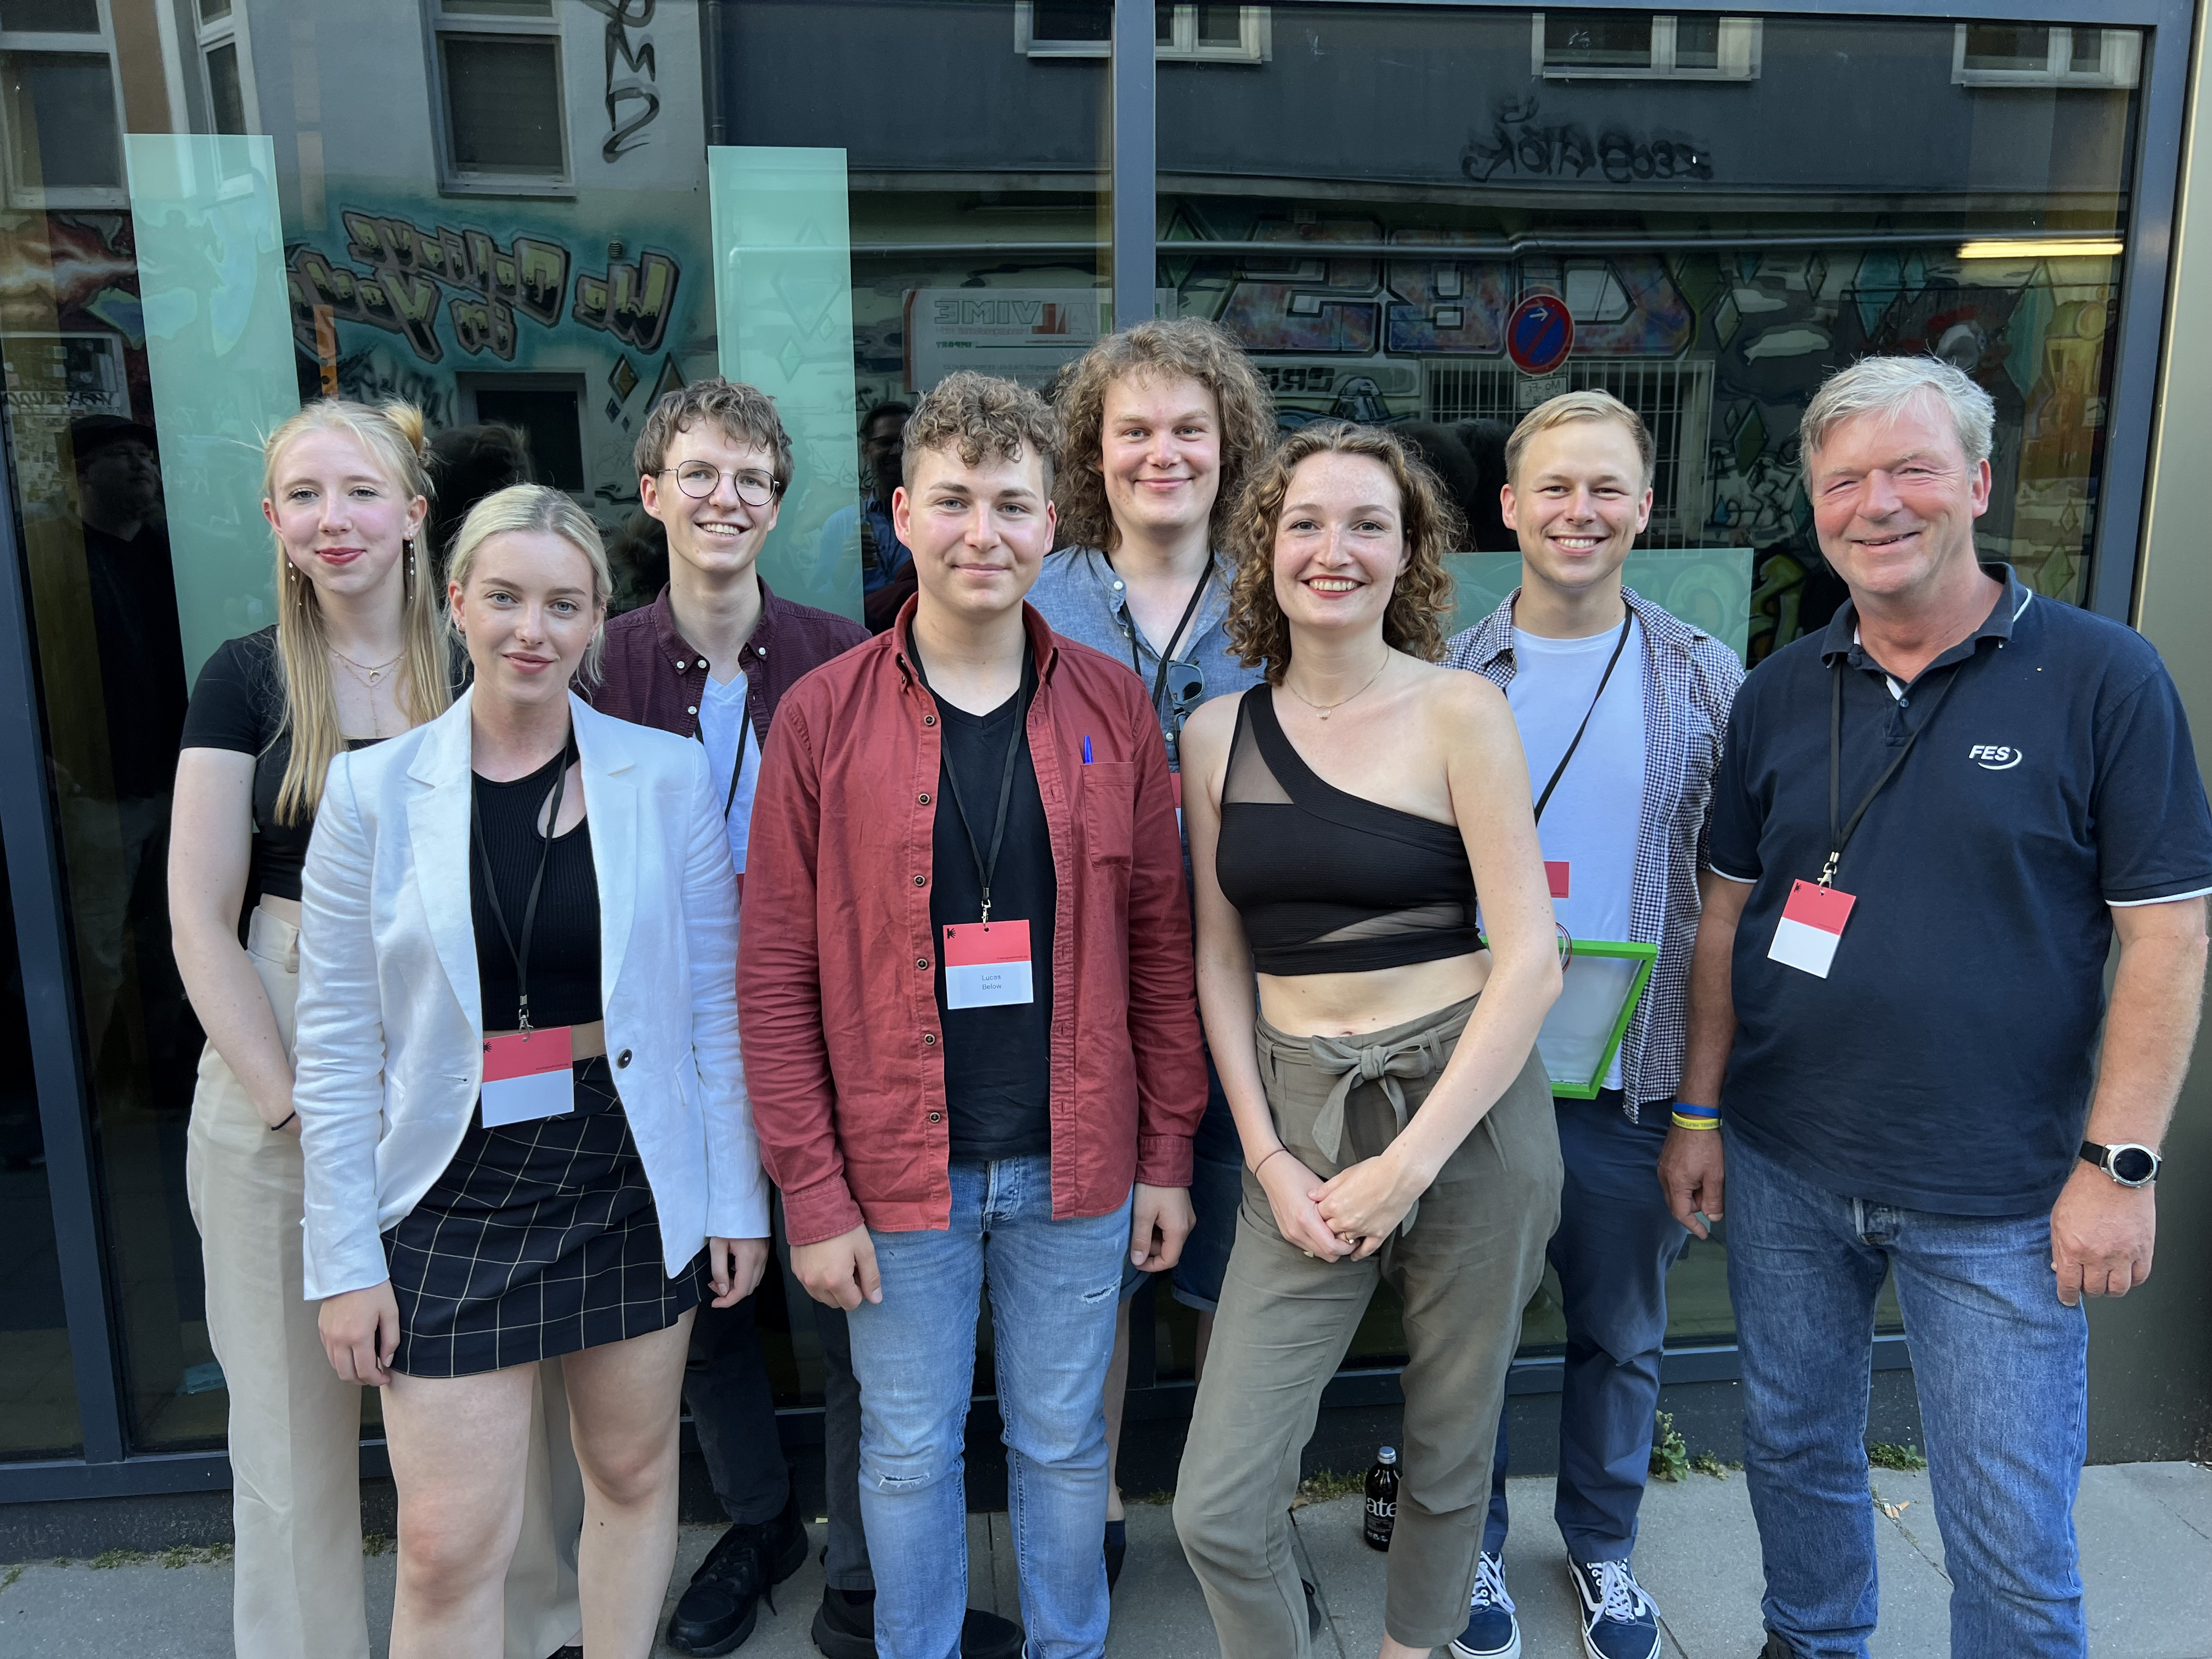
\includegraphics[width=12cm]{media/00_introduction/pic_team-FFM.jpg}
            \end{center}
            \caption[CIC Team Stadt Frankfurt]{CIC Team Stadt Frankfurt \par \small v.l.n.r.: Maybritt Braun (AMD), Annika Fröhlich (AMD), Robin von Berg (FHW), Lucas Below (AMD), Sven Hülsen (FHW), Celina Krug (HCU), Moritz Hillen (HCU), Jochen Schmitz (FES). Abwesend: Florian Bucher (HCU), Mechthild Schulze \& Karina Mombauer             (Stadt Frankfurt Stabstelle Digitalisierung)}
            \label{fig:team_frankfurt}
        \end{figure}

\section{Stadt Frankfurt - Stabstelle Digitalisierung}


    Beschreibung des Industriepartners


\section{Frankfurter Entsorgungs- und Service GmbH (FES)}

    Beschreibung des Industriepartners
